	\subsection{Closures} % (fold)
	\label{sub:closures}
	
	Umsetzung in Haskell

	\lstHaskell
	\begin{lstlisting}
obj = let x = 1
      in \() -> x <- x+1
	\end{lstlisting}

%%%
%%% end V10
%%%

%%%
%%% V11
%%%

		oder auch

		\lstHaskell
		\begin{lstlisting}
f = let a = 7 in \() -> a
		\end{lstlisting}

		ein Aufruf zeigt dann Folgendes

		\lstHaskell
		\begin{lstlisting}
f()
> 7
		\end{lstlisting}

		\begin{figure}[hb]
			\caption{Aufbau einer Haskell-Closure}
			
\includegraphics[width=\textwidth]{workfiles/v11_1}
		\end{figure}
		Hier liegt \texttt{var} liegt ausserhalb der Funktion \texttt{\textbackslash() -> a}. Die \texttt{var} müssen gültig sein.

		\lstHaskell[\texttt{let} in Haskell]
		\begin{lstlisting}
let a = 2
    b = 7
    ...
in ...
		\end{lstlisting}

		\lstLisp[\texttt{let} in Lisp]
		\begin{lstlisting}
(let ((v1 exp) (v2 exp)) e1 e2 ... en)
		\end{lstlisting}

		Bei obigem Beispiel ist en die Ausgabe bzw. das Ergebnis des Gesamtausdrucks.\\

		Variableneigenschaften in Lisp, Anm.: Hier fehlen die Live-Demos aus der Vorlesung.\\

		\begin{tabular}{rlll}
			& \textbf{Scope}	& \textbf{Extent} &  \\
		a	& lexical		& indefinite	& closures \\
		b	& indefinite	& dynamic		& special \\
		\end{tabular}$\;$\\

		Variablen festlegen in verschiedenen Sprachen:
		\begin{verbatim}
a := 150     Pascal
a = 150;     C
(setq a 150) Lisp
		\end{verbatim}

		\lstLisp[Spezialvariablen]
		\begin{lstlisting}
(declaim (special b))
		\end{lstlisting}

		Solche Spezialvariablen haben einen Stack von Werten, auf den beim Betreten von Scopes die Werte abgelegt werden.

		\lstHaskell[Anonyme Funktion]
	\begin{lstlisting}
\x -> x + x
		\end{lstlisting}

		\lstLisp[Anonyme Funktion]
		\begin{lstlisting}
(lambda (x) (+ x x))
		\end{lstlisting}

		\begin{figure}[H]
			\caption{Objekt-Aufbau in der ooP}
			
\includegraphics[width=\textwidth]{workfiles/v11_2}
		\end{figure}

		\begin{figure}[H]
			\centering
			\caption{Doppelbelegung von \texttt{max} (Live-Demo)}
			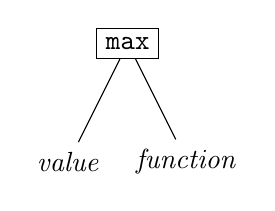
\begin{tikzpicture}
				\node [draw, rectangle] {\texttt{max}}
					child { node {\emph{value}}}
					child { node {\emph{function}}};
			\end{tikzpicture}
		\end{figure}
		(abhängig von der Situation wird die richtige Interpretation gewählt)
		Closures sind Grundlage für die ooP.
		
		\begin{figure}[H]
			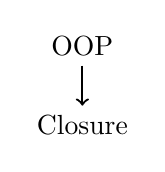
\begin{tikzpicture}
				\node (1) at (0,0) {OOP};
				\node (2) at (0,-1) {Closure};
				\path (1) edge [->,thick] (2);
			\end{tikzpicture}
		\end{figure}

	% subsection closures (end)

%%%
%%% end V11
%%%

%%%
%%% V12
%%%
\newpage
\subsection{Spezielle Variablen für Kommandointerpreter} % (fold)
\label{sub:spezielle_variablen_fuer_kommandointerpreter}

	\begin{tabular}{ll}
	+	&	letzter Ausdruck	\\
	++	&	vorletzter Ausdruck	\\
	+++	&	vorvorletzter Ausdruck
	\end{tabular}

	\begin{tabular}{ll}
	*	&	letzter Ergebnis	\\
	**	&	vorletzter Ergebnis	\\
	***	&	vorvorletzter Ergebnis
	\end{tabular}

	\begin{tabular}{ll}
	/	&	Liste mit letztem Ausdruck	\\
	//	&	Liste mit vorletztem Ausdruck	\\
	///	&	Liste mit vorvorletztem Ausdruck
	\end{tabular}

% subsection spezielle_variablen_fuer_kommandointerpreter (end)
\subsection{Makros} % (fold)
\label{sub:makros}

	Mechanismus, mit dem in Lisp Programme erstellt werden können\\
	\lstLisp[Programme als Syntaxbaum]
	\begin{lstlisting}
(+ ...)
	\end{lstlisting}

	Ist das erste Element eine Funktion (oben: Addition) $\Rightarrow$ Programm, sonst Liste
	\begin{itemize}
				\item Caching in Call-by-Name
				\item in Haskell
			\end{itemize}

	\subsubsection*{Auswertungsstrategien} % (fold)
	\label{ssub:auswertungsstrategien}

		\begin{tabular}{ll}
		Call-by-Value	&	strikte Asuwertung	\\
		Call-by-Name	&	nicht strikte Auswertung; lazy func. lang.\\
		\rotatebox[origin=c]{180}{$\Lsh$} Lazy-Evaluation	& $\rightarrow$ Caching in Call-by-Name\\
		&	$\rightarrow$ in Haskell
		\end{tabular}

		\begin{flalign*}
			&f(\perp)=\perp\qquad\qquad\text{CbV}\\
			&f(\perp)\neq\perp\qquad\qquad\text{CbN (kaum)}
		\end{flalign*}
	
	% subsubsection auswertungsstrategien (end)

	Wollen nun Funktion, die \texttt{a b c} nimmt und auch zurückliefert

	\lstLisp
	\begin{lstlisting}
(cond (1 a)
      (2 b)
      (3 b))
(defun f (a b c) (list 'cond (list 1 a)
                             (list 2 b)
                             (list 3 c)))
	\end{lstlisting}

	Das wird kompliziert...\\
	Mit Template durch Backquote \texttt{`}:

	\lstLisp
	\begin{lstlisting}
`(cond (1 ,a)
       (2 ,b)
       (3 ,c))
(defun f (a b c) `(cond (1 ,a)
                        (2 ,b)
                        (3 ,c)))
	\end{lstlisting}

	\lstLisp[Verzweigungen]
	\begin{lstlisting}
(if <cond> <then> <else>)

(cond ((<cond> <expr>)
       ...
       (<cond> <expr>)))
	\end{lstlisting}

	\lstFortran[arithmetisches If in Fortan]
	\begin{lstlisting}
IF <exp>
	< 0	F1
	= 0	F2
	> 0	F3
	\end{lstlisting}

	\lstLisp[arithmetisches If in Lisp]
	\begin{lstlisting}
((let ((v <expr>))
 (cond (cond (( v<0 ) F1))
       (cond (( v=0 ) F2))
       (cond (( v>0 ) F3)))))
	\end{lstlisting}

	Lieber wäre uns ein Aufbau wie

	\lstLisp
	\begin{lstlisting}
(aif <c> <F1> <F2> <F3>)
	\end{lstlisting}

	geht auch:

	\lstLisp
	\begin{lstlisting}
(defmacro aif (c F1 F2 F3))
	\end{lstlisting}

	\lstLisp
	\begin{lstlisting}
`(cond ((minusp ,c) F1)
       ((zerop ,c) F2)
       ((plusp ,c) F3))
	\end{lstlisting}

% subsection makros (end)

%%%
%%% end V12
%%%

%%%
%%% V13
%%%

\subsection{Common Lisp Object System (CLOS)} % (fold)
\label{sub:common_lisp_object_system_}
	
	\begin{figure}[H]
		
\begin{tikzpicture}
			\node (1) at (0,0) {CLOS};
			\node (2) at (2,0) {LISP};
			\path (1) edge [->,thick] (2);
		\end{tikzpicture}
	\end{figure}
	via Makros und Struct\\

	In Haskel arbeiten wir mit 
	\lstHaskell
	\begin{lstlisting}
data ... deriving Show
	\end{lstlisting}
	und rufen damit \texttt{Show} in der jeweiligen Instanz auf\\

	In Lisp wird
	\lstLisp
	\begin{lstlisting}
defmethod print-object
	\end{lstlisting}
	aufgerufen, wenn ein Objekt ausgegeben werden soll.

	\subsubsection*{Vererbungshierarchie} % (fold)
	\label{ssub:vererbungshierarchie}
		
		\begin{figure}[H]
			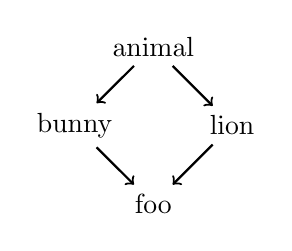
\begin{tikzpicture}
				\node (1) at (0,0) {animal};
				\node (2) at (-1,-1) {bunny};
				\node (3) at (1,-1) {lion};
				\node (4) at (0,-2) {foo};
				\path (1) edge [->,thick] (2);
				\path (1) edge [->,thick] (3);
				\path (2) edge [->,thick] (4);
				\path (3) edge [->,thick] (4);
			\end{tikzpicture}
		\end{figure}
		Bei Mehrfachvererbung wird die Reihenfolge entscheident
		
		\begin{figure}[H]
			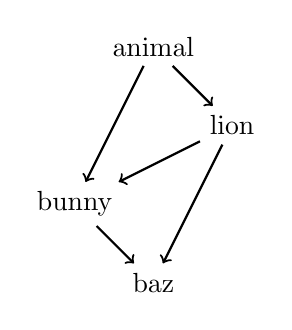
\begin{tikzpicture}
				\node (1) at (0,0) {animal};
				\node (2) at (-1,-2) {bunny};
				\node (3) at (1,-1) {lion};
				\node (4) at (0,-3) {baz};
				\path (1) edge [->,thick] (2);
				\path (1) edge [->,thick] (3);
				\path (3) edge [->,thick] (2);
				\path (2) edge [->,thick] (4);
				\path (3) edge [->,thick] (4);
			\end{tikzpicture}
		\end{figure}

	% subsubsection vererbungshierarchie (end)

	\subsubsection*{Methodenaufrufe bei Vererbung} % (fold)
	\label{ssub:methodenaufrufe_bei_vererbung}

		\begin{figure}[h]
			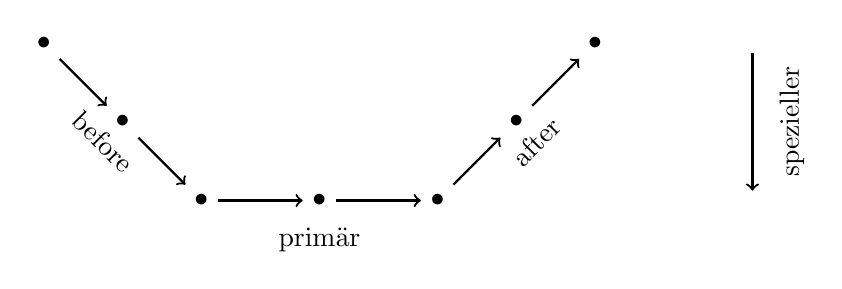
\begin{tikzpicture}
				\node (1) at (0,0) {$\bullet$};
				\node (2) at (1,-1) {$\bullet$};
				\node (3) at (2,-2) {$\bullet$};
				\node (4) at (3.5,-2) {$\bullet$};
				\node (5) at (5,-2) {$\bullet$};
				\node (6) at (6,-1) {$\bullet$};
				\node (7) at (7,0) {$\bullet$};

				\node (8) at (3.5,-2.5) {primär};
				\node (9) at (0.75,-1.25) {\rotatebox[origin=c]{-45}{before}};
				\node (10) at (6.25,-1.25) {\rotatebox[origin=c]{45}{after}};

				\node (11) at (9,0) {};
				\node (12) at (9,-2) {};

				\node (13) at (9.5,-1) {\rotatebox[origin=c]{90}{spezieller}};

				\path (1) edge [->,thick] (2);
				\path (2) edge [->,thick] (3);
				\path (3) edge [->,thick] (4);
				\path (4) edge [->,thick] (5);
				\path (5) edge [->,thick] (6);
				\path (6) edge [->,thick] (7);

				\path (11) edge [->,thick] (12);
			\end{tikzpicture}
		\end{figure}
	
	% subsubsection methodenaufrufe_bei_vererbung (end)


% subsection common_lisp_object_system_ (end)

%%%
%%% end V13
%%%